%********************************************************************************
% Title: A performance modeling showcase
%
% Series: Courseworks in Performance Modeling of Computer Systems and Networks
%
% Author: Giacomo Marciani <gmarciani@acm.org>
%
% Institution: Department of Civil Engineering and Computer Science Engineering,
% University of Rome Tor Vergata, Italy
%
% Style: ACM ART SIGCONFS (based on ACM Large v1.7)
%*******************************************************************************

\documentclass[sigconf]{acmart}

\usepackage[utf8]{inputenc}
\usepackage{booktabs}
\usepackage{algorithm2e}
\usepackage{listings}
\usepackage{color, soul}
\usepackage{graphicx}
\usepackage{lipsum}
\usepackage{epstopdf}
\usepackage{subfig}
\usepackage{bm}
\usepackage{url}
\usepackage{array}

%*******************************************************************************
% Packages setting
%*******************************************************************************
\graphicspath{{fig/}}

%*******************************************************************************
% Shared Affiliation format
%*******************************************************************************
\def\sharedaffiliation{%
\end{tabular}
\begin{tabular}{c}}

%*******************************************************************************
% Fonts
%*******************************************************************************
%\newfont{\eaddfntresz}{phvr8t at 11pt}

%*******************************************************************************
% Margins
%*******************************************************************************
%\clubpenalty=10000
%\widowpenalty=10000

%*******************************************************************************
% hyphenation
%*******************************************************************************
\hyphenation{sched-uler par-a-digm adopt-ed evolv-ing th}

%*******************************************************************************
% pseudocode customisation
%*******************************************************************************
%\makeatletter
%\def\BState{\State\hskip-\ALG@thistlm}
%\makeatother

%*******************************************************************************
% Details
%*******************************************************************************
\acmConference[PMCSN'18]{A Performance Modeling Showcase}{January 2018}{Rome, Italy}
\acmYear{2018}
\copyrightyear{2018}
\setcopyright{rightsretained}
\acmISBN{123-4567-24-567/08/06}
\acmDOI{10.475/123_4}
\acmPrice{15.00}

\begin{document}
%*******************************************************************************
% Title
%*******************************************************************************
\title{A Performance Modeling Showcase}

%*******************************************************************************
% Authors
%*******************************************************************************
\author{Giacomo Marciani}
\orcid{0000-0002-3675-8804}
\affiliation{%
  \institution{University of Rome Tor Vergata}
  \streetaddress{Via del Politecnico 1}
  \city{Rome}
  \state{Italy}
  \postcode{00133}
}
\email{gmarciani@acm.org}

% The default list of authors is too long for headers}
\renewcommand{\shortauthors}{G. Marciani}

%*******************************************************************************
% Contents
%*******************************************************************************
\begin{abstract}
It has been previously proposed that understanding the mechanisms of
contour perception can provide a theory for why some flow-rendering
methods allow for better judgments of advection pathways than others.
In the present article, we develop this theory through a numerical
model of the primary visual cortex of the brain (Visual Area 1) where
contour enhancement is understood to occur according to most
neurological theories. We apply a two-stage model of contour
perception to various visual representations of flow fields evaluated
using the advection task of Laidlaw et al. [2001]. In the first
stage, contour {enhancement} is modeled based on Li's cortical model
[Li 1998]. In the second stage, a model of streamline {tracing} is
proposed, designed to support the advection task. We examine the
predictive power of the model by comparing its performance to that of
human subjects on the advection task with four different
visualizations. The results show the same overall pattern for humans
and the model. In both cases, the best performance was obtained with
an aligned streamline-based method, which tied with a LIC-based
method. Using a regular or jittered grid of arrows produced worse
results. The model yields insights into the relative strengths of
different flow visualization methods for the task of visualizing
advection pathways.
\end{abstract}

% CCS keywords are generated by http://dl.acm.org/ccs.cfm

\begin{CCSXML}
	<ccs2012>
	<concept>
	<concept_id>10010147.10010341.10010366.10010369</concept_id>
	<concept_desc>Computing methodologies~Simulation tools</concept_desc>
	<concept_significance>500</concept_significance>
	</concept>
	</ccs2012>
\end{CCSXML}

\ccsdesc[500]{Computing methodologies~Simulation tools}

\keywords{performance modeling; queueing theory; web service simulation; random number generation; randomness analysis}
\maketitle
\section{Introduction}
\label{sec:introduction}


% %
% WORK INTRODUCTION
% %
As computing is getting more ubiquitous in our lives, computer infrastructures are getting increasingly complex and software applications are required to meet high level performance.

%
% %
% PROBLEM STATEMENT
% %
In this context, knowing how to design and optimize computer systems and networks is one of the most important skills for software engineers and a strategic asset for companies, both in terms of technology and investments.
%
% %
% APPROACH
% %
In this technical report we propose a next-event simulator to analyze the performance of a two-layers Fog-like system that serves classed workloads and leverages an off-loading policy between its layers.


% %
% PAPER ORGANIZATION
% %
The remainder of the paper is organized as follows.
%
In Section~\ref{sec:system} we give an high level description of the target system.
%
In Section~\ref{sec:random-number-generation} we describe the pseudo-random number generator adopted to generate random variates for the next-event simulation model.
%
In Section~\ref{sec:performance-modeling} we describe the the next-event simulation model in terms of goals, conceptual model, specification model, computational model, verification and validation.
%
In Section~\ref{sec:evaluation} we show the experimental results about both the randomness of the adopted pseudo-random number generator and the performance analysis of the target system conducted leveraging our simulator.
%
In Section~\ref{sec:usage} we show how to configure and run experiments and give some sample outputs to provide a better idea of what has been created.
%
In Section~\ref{sec:conclusions} we conclude the paper summing up the work that has been done and delineating future improvements.

\section{Random number generation}
\label{sec:random-number-generation}

The generation of pseudo-random numbers is a fundamental building-block for next-event simulations.
%
In fact, a sequence of pseudo-random numbers uniformly distributed in $(0,1)$ can be used to generate stochastic variates, e.g. the exponential distribution, that can be leveraged to generate random stream of events, e.g. requests to the system with random occurrence time and computational demand.
%
There exist many techniques for random number generation, a lot of which are comprehensively presented in \cite{l1994uniform}.
The most notable algorithmic generators are \textit{multiple recursive generators}, \textit{composite generators}, and \textit{shift-register generators}.
Although all of these produce periods wider than the one produced by a Lehmer generator, they also have a sensible cost in terms of computational complexity.

In this work we adopted a multi-stream Lehmer generator $(a,m,s)$, which is defined by the following equation,

\begin{equation}
\label{eqn:lehmer}
x_{i+1} = (a^{j} \mathrm{mod}m) x_{i} \mathrm{mod}m \qquad\forall j=0,...,s-1
\end{equation}

where $m$ is the modulus, $a$ is the multiplier, $s$ is the number of streams and $(a^{j} \mathrm{mod}m)$ is the jump multiplier.

We have chosen this solution because (i) it provides a great degree of randomness with the appropriate parameters (ii) the multi-streaming is required by simulations with multiple stochastic components (iii) it is a de-facto standard, hence it is easy to compare our experimental results with the one provided in literature.

We propose a generator with the following parameters:

\begin{itemize}
	\item \textbf{modulus $\mathbf{2^{31}-1}$:} the modulus should be the maximum prime number that can be represented in the target system. 
	Although all modern computers have a 64-bit architecture, we considered a 32-bit one because the algorithm to find the right multiplier for a 64-bit modulus can be very slow.
	For this reason we have chosen $2^{31}-1$ as our modulus.
	
	\item \textbf{multiplier $\mathbf{50812}$:} the multiplier should be \textit{full-period modulus-compatible} with respect to the chosen modulus. The chosen modulus has 23093 of such multipliers. Among these there are also multipliers such $16807$, widely used in the past, and $48271$, that is currently the most widely adopted.
	We have chosen $50812$ as our multiplier because we wanted to study a suitable multiplier that is different from the de-facto standard.
	
	\item \textbf{$\mathbf{256}$ streams:} the original periodic random sequence can be partitioned in different disjoint periodic random subsequences, one for each stream. 
	The number of streams should be no more than the number of required disjoint subsequences, because streams come with the cost of reducing the size of the sequence.
	We have chosen 256 streams, that is a lot more than the strictly required for our simulations, because it is a de-facto standard hence it is useful for comparisons between our evaluation and the one proposed in \cite{leemis2006discrete}.
	
	\item \textbf{jump multiplier $\mathbf{29872}$:} the jump multiplier is used to partition the random sequence in disjoint subsequences, one for each stream, whose length is often called jump size. The jump multiplier should be modulus compatible with he chosen modulus.
	We have chosen $29872$ as our jump multiplier because it is the value that maximizes the jump size.
	
	\item \textbf{initial seed $\mathbf{123456789}$:} the initial seed is the starting point of the finite sequence of generated values. Even if the initial seed does not impact the randomness degree of a generator in a single run (it only has to be changed in different replication of the same enseble), we decide to indicate it here for completeness. 
\end{itemize}

The randomness degree of such a generator has been assessed by the usage of \textit{spectral test}, \textit{test of extremes} and the \textit{analysis of Kolomogorv-Smirnov}.
%
The experimental results are reported in Section~\ref{sec:evaluation}.

\section{Modeling}
\label{sec:modeling}


% %
% SYSTEM DESCRIPTION
% %
We consider the environment sketched in Figure~\ref{fig:modeling-system-sketch}, which is characterized by:

\begin{itemize}
	\item  \textbf{workload:} mobile devices send to the system tasks that can be partitioned in two classes $C_{1}$ and $C_{2}$.
	\item \textbf{system:} a two-tiers system, made of:	
	\begin{itemize}
		\item a remote Cloud server with virtually unlimited servants.
		\item a Cloudlet with $N$ servants, having the ability to off-load tasks to the Cloud, accordingly to a certain \textit{off-loading policy} parametrized by a given \textit{threshold}.
	\end{itemize}
\end{itemize}

\begin{figure}
	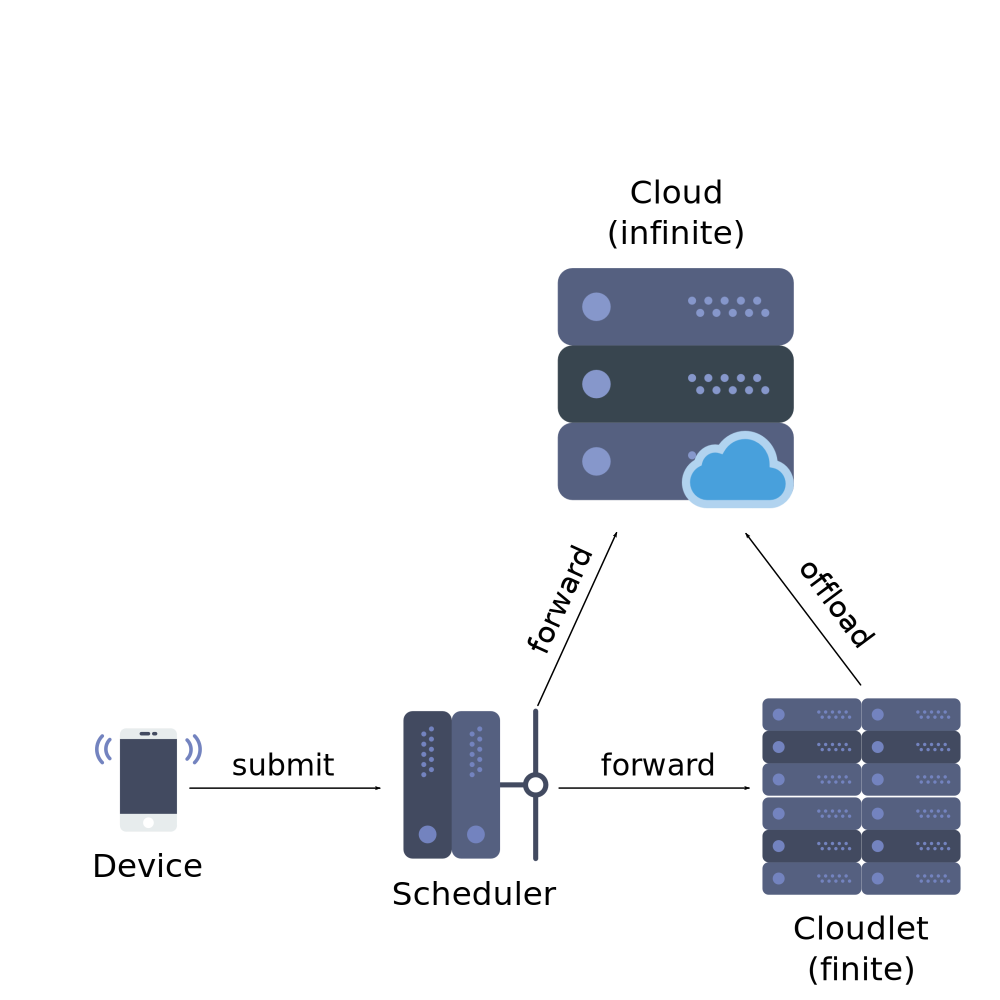
\includegraphics[width=\columnwidth]{fig/modeling-system-sketch}
	\caption{The system sketch.}
	\label{fig:modeling-system-sketch}
\end{figure}

We assume that
(i) the Cloudlet provides tasks with higher service rate than the Cloud, 
(ii) when a task is interrupted in the Cloudlet and it is sent to the Cloud, the restart process comes with a \textit{setup time overhead}.

% %
% GOALS AND OBJECTIVES
% %
\paragraph{Goals and Objectives}
The main goals of the simulation are about system tuning.
In particular, we propose to determine with a $95\%$ level of confidence
\begin{itemize}
	\item the response time as a function of the threshold $S$,
	\item the throughput as a function of the threshold $S$,
	\item the distribution of the response time when $S=N$ and
	\item the threshold of the off-loading policy that minimizes the response time.
\end{itemize}


% %
% CONCEPTUAL MODEL
% %
\paragraph{Conceptual Model}
The conceptual model is depicted in Figure~\ref{fig:modeling-conceptual-model}.

\begin{figure}
	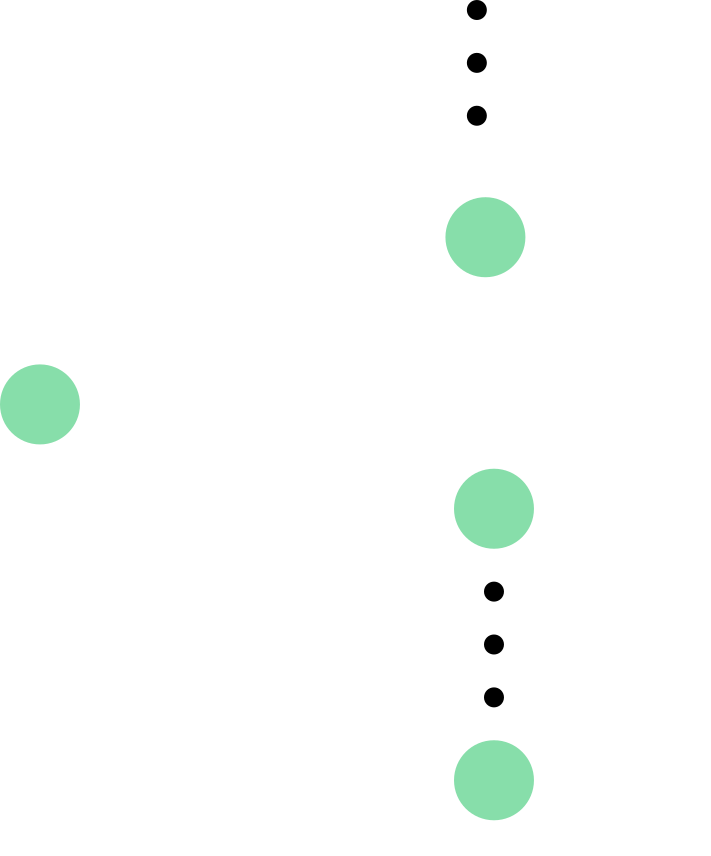
\includegraphics[width=\columnwidth]{fig/modeling-conceptual-model}
	\caption{The conceptual model.}
	\label{fig:modeling-conceptual-model}
\end{figure}

% %
% SPECIFICATION MODEL
% %
\paragraph{Specification Model}
The state of a system is a comprehensive characterization of the system at a particular time.
The state of the system is represented by the pair $(n_{clt,1},n_{clt,2},n_{cld,1},n_{cld,2})$, where $n_{cld,i}$ is the number of tasks belonging to the $i$-th class within the Cloudlet and $n_{cld,i}$ is the number of tasks belonging to the $i$-th class within the Cloud.
An event is an occurrence that could change the state of the system at the event time, according to the event type.
Our events are ...

Tasks belonging to the first class, i.e. $t\in C_{1}$ arrive to the system with an exponential arrival process with rate $ \lambda_{1}$; whilst tasks belonging to the seconds class, i.e. $t\in C_{2}$ arrive to the system with an exponential arrival process with rate $ \lambda_{2}$.
The Cloudlet serves tasks belonging to the first class with exponentially distributed service time with rate $\mu_{cld,1}$; whilst the Cloudlet serves tasks belonging to the second class with exponentially distributed service time with rate $\mu_{cld,2}$.
The Cloud serves tasks belonging to the first class with exponentially distributed service time with rate $\mu_{clt,1}$; whilst the Cloudlet serves tasks belonging to the second class with exponentially distributed service time with rate $\mu_{clt,2}$.
We assume that 
(i) $\mu_{clt,i}>\mu_{cld,i}\ \forall i=1,2$ and
(ii) the setup time $T_{setup}$ is exponentially distributed with expected value $E[T_{setup}]$.

\begin{algorithm}
	\SetAlgoLined
	\If{task of class 1}{
		\If{$n_{clt}=N$}{
			send on the Cloud
		} 
		\If{$n_{clt}+n_{cld}<S$}{
			accept
		} 
		\eIf{$n_{cld} > 0$}{
			accept the task on the Cloudlet and send a class 2 task on the Cloud
		}{
		accept the task on the Cloudlet
		}
	}
	\If{arrival of class 2}{
		\eIf{$n_{clt}+n_{cld}>=S$}{
			send on the Cloud
		}{
		accept the task on the Cloudlet
	}
	}
	\caption{The dispatching policy.}
	\label{alg:modeling-dispatching-policy}
\end{algorithm}

% %
% COMPUTATIONAL MODEL
% %
\paragraph{Computational Model}
The proposed performance model has been implemented as a Python application. 
The simulation parameters can be configured with a simple YAML file that can be loaded by the simulation program.
The full open source code is available at \cite{gmarciani-pydes} and some representative configurations and outputs are presented in Section~\ref{sec:usage}.

We adopted the next-event simulation paradigm, using 
(i) a custom multi-stream Lehmer generator to generate random events, whose parameters have been described in Section~\ref{sec:random-number-generation} and whose evaluation will be presented in Section~\ref{sec:evaluation}; and
(ii) a priority-queue based calendar with the ability both to schedule and un-schedule events.

Even if both the initial and terminal state can have any possible value, we adopted the convention of initializing and terminating the system in the idle state $(0,0,0,0)$. In particular, the terminal state is reached via the well-known closed door technique driven by a stop time condition.

The calendar is initialized by scheduling the first arrival in the initialization phase. The submission of an arrival $a$ to the system could induce
(i) the scheduling of the corresponding completion event,
(ii) the scheduling of a new arrival, or
(iii) the unscheduling of a previously scheduled completion, i.e. interruption in Cloudlet.

The next-event calendar is implemented as priority queue, appropriately extended to manage scheduling/unscheduling of events and exclusion of impossible events, i.e. arrivals with occurrence time greater than the stop time.
The impossibility of events is managed by letting the calendar contain possible events only, which is the best approach when the event list is assumed to be very long.


% %
% VERIFICATION
% %
\paragraph{Verification}
The verification has been carried out taking into account two dimensions: we verified the computational model by (i) checking the consistency of its response to input variations and (ii) checking the comparison of the computed performance indices with the ones calculated with a theoretical model.
%
In particular, the model has been verified by 
\begin{itemize}
	\item \textbf{flow consistency:} verifies the correctness of flow trends, such as:
	
	\begin{equation}
	n_{cld,i}=a_{cld,i}-c_{cld,i}-s_{cld,i}
	\end{equation}
	\begin{equation}
	n_{cld,i}=a_{cld,i}-c_{cld,i}+s_{cld,i}
	\end{equation}
	\begin{equation}
	s_{clt,i}=s_{cld,i}
	\end{equation}
	
	where 
	$n_{j,i}$ is the population of tasks belonging to $i$-th class in the $j$-th subsystem, 
	$a{j,i}$ is the number of tasks belonging to $i$-th class arrived to the $j$-th subsystem, 
	$c{j,i}$ is the number of tasks belonging to $i$-th class completed in the $j$-th subsystem, 
	$s{j,i}$ is the number of tasks belonging to $i$-th class switched from/to the $j$-th subsystem.
	 
	\item \textbf{workload change consistency:} verifies the correctness of metrics variations in response to arrival/service rates variations, such as:
	
	\begin{equation}
		\lambda_{1}' > \lambda_{1} \Rightarrow
	\end{equation}
	
	\item \textbf{stationary check:} responsible to verify the correctness of the model in stationary conditions leveraging the Continuous Time Markov Chain model.
\end{itemize}

% %
% VALIDATION
% %
\paragraph{Validation}
It is well-known that model development should include a final validation step in order to assess the consistency of the model with the real system. 
%
As the simulation main purpose is insight, a widely adopted technique is to place the computational model alongside with the real system and check the consistency of performance indices.
%
Clearly, we cannot conduct this final step because we cannot compare the performance model with its real counterpart.
%
For this reason, we totally rely on the verification step, considering the calculus made on the theoretical model (e.g. leveraging Markov Chains) as the best alternative available to us
\section{Evaluation}
\label{sec:evaluation}

In this Section, we present our experimental results.
First, we show the results about the randomness degree of the adopted pseudo-random number generator.
Then, we show the results about the performance recorded by the simulation of the target system.

% %
% EXPERIMENTAL ENVIRONMENT
% %
The experiments have been conducted on an Amazon EC2 c3.8xlarge instance, which is really indicated for high performance science and engineering applications\footnote{https://aws.amazon.com/ec2/instance-types/}.
The instance is equipped with 32 vCPU based on an Intel Xeon E5-2680 v2 (Ivy Bridge) processor, 30 GB of RAM and SSD with 900 IOPS.
It runs Debian 8.3 (Jessie), Python 3.5.2, and the Python-ported version of the official Leemis library for discrete-event simulation, indicated in \cite{leemis2006discrete}.
Our solution has been developed in Python, following the de-facto standard best-practices, stated in \cite{reitz2016,GooglePythonStyleguide}.

% %
% RANDOMNESS ANALYSIS
% %
\subsection{Randomness Analysis}
\label{sec:evaluation-randomness-analysis}
Let us now consider the results about the randomness degree of the adopted generator.
The randomness has been assessed by the following tests:

\begin{itemize}
	\item \textbf{Spectral Test:} this test is considered one of the most powerful tests to assess the quality of linear congruential generators \cite{knuth1981art}. It relies on the fact that the output of such generators form lines or hyperplanes when plotted on 2 or more dimensions. The less the distance between these lines or planes, the better the generator is. In fact, a smaller distance between lines or planes highlights a better uniform distribution.
	
	In Figure~\ref{fig:experimental-analysis-randomness-spectral-16807,fig:experimental-analysis-randomness-spectral-48271,fig:experimental-analysis-randomness-spectral-58012} we show the test results for generators $(16807,2^{31}-1)$, $(48271,2^{31}-1)$ and $(50812,2^{31}-1)$, respectively.
	
	The results show that our generator $(50812,2^{31}-1)$ is much better than $(16807, 2^{31}-1)$, which was a past de-facto standard, and it is really similar to $(48271,2^{31}-1)$, which is the current de-facto standard, according to \cite{leemis2006discrete}.
	
	\item \textbf{Test of Extremes:} this test relies on the fact that if $U=U_{0},...,U_{d-1}$ is an independent identically distributed sequence of $Uniform(0,1)$ random variables, then $\max(U)^{d}$ is also a $Uniform(0,1)$. The test leverages this property to measures, for every stream, how much the generated random values differ from the theoretical uniform distribution.
	
	Given a number of streams $s$ and a level of confidence $c=1-\alpha$, the more the total number of fails is close to the expected value, i.e. $s \cdot c$, the better the generator is.
	
	In Figure~\ref{fig:experimental-analysis-randomness-extremes-50812} we show the test results for the proposed generator $(508012,2^{31}-1, 256)$ with sample size $n=10000$, $k=1000$ bins, sequence size $d=5$ and $95\%$ level of confidence.
	%	
	The proposed generator shows critical values $v_{min}=913$ and $v_{max}=1088$ and 14 total fails (7 lower fails and 7 upper fails), that is not far from the theoretical accepted number of fails, i.e. $256*0.05=13$.
	The proposed generator successfully passed the test with a $94.531\%$ level of confidence.
	
	\item \textbf{Kolmogorov-Smirnov Analysis:} the test measures, at a given level of confidence, the biggest vertical distance between the theoretical cumulative distribution function and the empirical cumulative distribution function.
	The more the recorded distance $d$ is less than the critical value $d*$ for the considered level of confidence, the better the generator is.
	As the Kolmogorov-Smirnov analysis relies on pre-calculated randomness statistics, we have chosen to take into account the statistics obtained by the previous test.
	
	In Figure~\ref{fig:evaluation-randomness-kolmogorov-smirnov-50812} we show the test results for the proposed generator $(50812,2^{31}-1, 256)$ with a $95\%$ level of confidence.
	%
	The proposed generator successfully passed the test, as $d=0.041<0.081=d*$.
	
\end{itemize}

\begin{figure}
	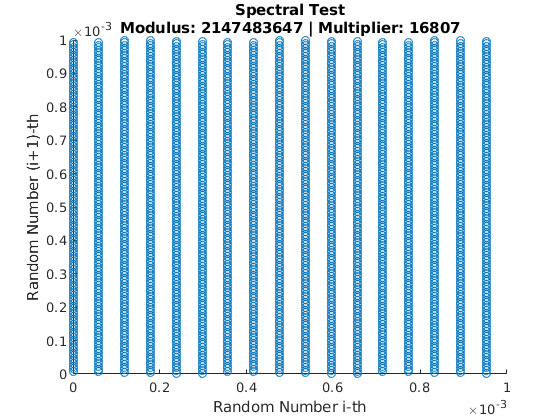
\includegraphics[width=\columnwidth]{fig/evaluation-randomness-spectral-16807}
	\caption{The Spectral Test to evaluate the randomness of the random number generator $(16807,2^{31}-1, 1)$ in the interval $(0, 10^{-3})$.}
	\label{fig:evaluation-randomness-spectral-16807}
\end{figure}

\begin{figure}
	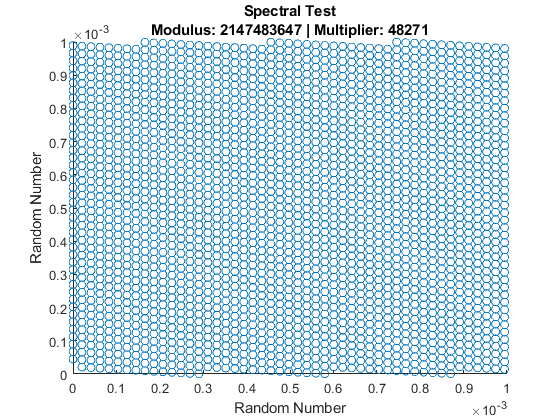
\includegraphics[width=\columnwidth]{fig/evaluation-randomness-spectral-48271}
	\caption{The Spectral Test to evaluate the randomness of the random number generator $(48271,2^{31}-1, 1)$ in the interval $(0, 10^{-3})$.}
	\label{fig:evaluation-randomness-spectral-48271}
\end{figure}

\begin{figure}
	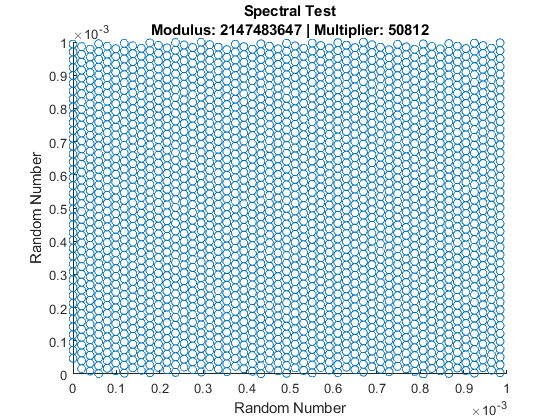
\includegraphics[width=\columnwidth]{fig/evaluation-randomness-spectral-50812}
	\caption{The Spectral Test to evaluate the randomness of the random number generator $(50812,2^{31}-1, 1)$ in the interval $(0, 10^{-3})$.}
	\label{fig:evaluation-randomness-spectral-50812}
\end{figure}

\begin{figure}
	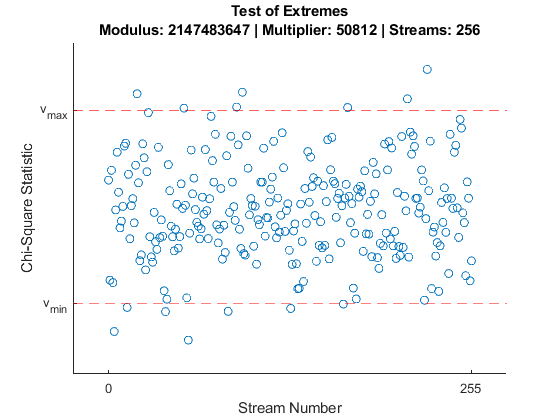
\includegraphics[width=\columnwidth]{fig/evaluation-randomness-extremes-50812}
	\caption{The Test of Extremes with $d=5$ to evaluate the randomness of the random number generator $(50812,2^{31}-1, 256)$.}
	\label{fig:evaluation-randomness-extremes-50812}
\end{figure}

\begin{figure}
	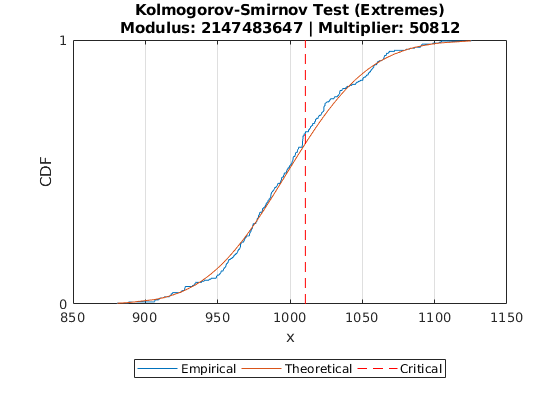
\includegraphics[width=\columnwidth]{fig/evaluation-randomness-kolmogorov-smirnov-50812}
	\caption{The Kolmogorov-Smirnov Analysis (leveraging the Test of Extremes with $d=5$) to evaluate the randomness of the random number generator $(50812,2^{31}-1, 256)$ with $0.95$ confidence level.}
	\label{fig:evaluation-randomness-kolmogorov-smirnov-50812}
\end{figure}


% %
% PERFORMANCE ANALYSIS
% %
\subsection{Performance Analysis}
Let us now consider the results about the performance recorded during the simulation of the target system.
In all experiments we considered values stated in Section~\ref{sec:performance-modeling}.

\subsection{Transient Analysis}
\label{sec:evaluation-transient-analysis}
First, we conduct a \textit{transient analysis} to evaluate the stationary of the system and to estimate the duration of the transient period.
%
In fact, given a system that converges to stationary, the knowledge of the duration of the transient period is really important to conduct an effective performance evaluation. In particular, it allows the analyst to focus performance evaluation on a system in its stationary conditions.
%
In the transient analysis we focus on the following global metrics for the whole system: response time, throughout, mean population, ratio of switched tasks, response time for switched tasks. 
%
We assess the transient period of the aforementioned metrics because they are also the performance metrics that will be taken into account in the final performance evaluation, thus it is really important to study their stationary.

The following results have been produced by considering an ensemble of $5$ replications, where the $i+1$-th replication is initialized with the last seed of the $i$-th replication, so as to achieve the best decoupling between random sequences of different replications.

In Figure \ref{fig:evaluation-transient-analysis-response-time} we show the transient analysis of the global response time in the whole system.
%
In Figure \ref{fig:evaluation-transient-analysis-throughput} we show the transient analysis of the global throughput in the whole system.
%
In Figure \ref{fig:evaluation-transient-analysis-mean-population} we show the transient analysis of the global mean population in the whole system.
%
In Figure \ref{fig:evaluation-transient-analysis-switched-ratio} we show the transient analysis of the global switch ratio in the whole system.
%
In Figure \ref{fig:evaluation-transient-analysis-switched-response-time} we show the transient analysis of the response time for switched tasks in the whole system.

The results show that 
(i) the system is stationary,
(ii) the response time, the throughput, the mean population and the ratio of switched tasks loose their dependence on the starting conditions, whilst 
(iii) the response time for switched tasks maintains its dependence on starting conditions, regardless of the termination of the transient period.

As we could image, each metric exposes a distinct transient period, e.g. the ratio of switched tasks converges faster than the mean population. Thus, we consider $\tau*=8\cdot 10^{4}\;sec$ as the final instant of the transient period, as in $\tau*$ we are sure that all metrics loosed their dependence on starting conditions.

\begin{figure}
	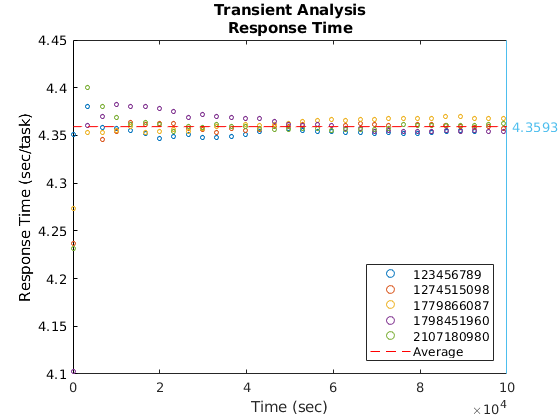
\includegraphics[width=\columnwidth]{fig/evaluation-transient-analysis-response-time}
	\caption{Transient analysis for global response time in the whole system.}
	\label{fig:evaluation-transient-analysis-response-time}
\end{figure}

\begin{figure}
	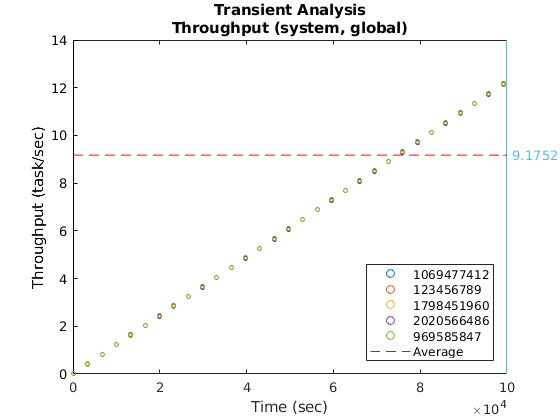
\includegraphics[width=\columnwidth]{fig/evaluation-transient-analysis-throughput}
	\caption{Transient analysis for global throughput in the whole system.}
	\label{fig:evaluation-transient-analysis-throughput}
\end{figure}

\begin{figure}
	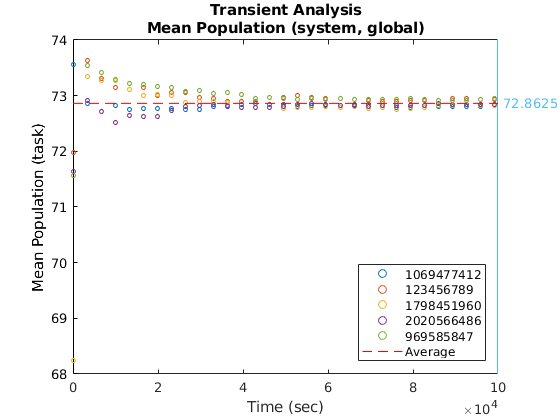
\includegraphics[width=\columnwidth]{fig/evaluation-transient-analysis-mean-population}
	\caption{Transient analysis for global mean population in the whole system.}
	\label{fig:evaluation-transient-analysis-mean-population}
\end{figure}

\begin{figure}
	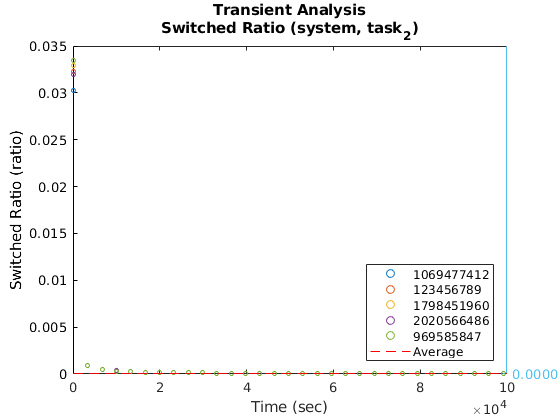
\includegraphics[width=\columnwidth]{fig/evaluation-transient-analysis-switched-ratio}
	\caption{Transient analysis for the ratio of switched tasks of type 2.}
	\label{fig:evaluation-transient-analysis-switched-ratio}
\end{figure}

\begin{figure}
	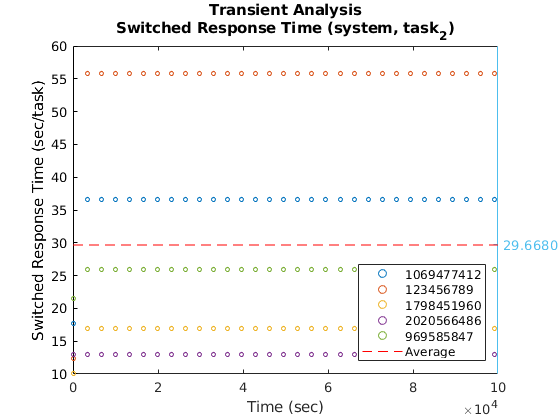
\includegraphics[width=\columnwidth]{fig/evaluation-transient-analysis-switched-response-time}
	\caption{Transient analysis for response time for switched tasks of type 2.}
	\label{fig:evaluation-transient-analysis-switched-response-time}
\end{figure}


\subsection{Performance Evaluation}
Let us now focus on the \textit{performance evaluation}, taking into account the following metrics:

\begin{enumerate}
	\item response time both global and per-class, both for the system as a whole and for each subsystem;
	\item throughput both global and per-class, both for the system as a whole and for each subsystem;
	\item mean population both global and per-class, both for the system as a whole and for each subsystem;
	\item ratio of switched tasks of type 2;
	\item response time for switched tasks of type 2.
\end{enumerate}

\begin{figure}
	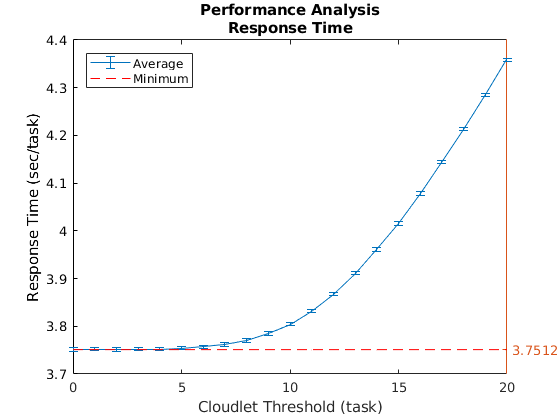
\includegraphics[width=\columnwidth]{fig/evaluation-performance-analysis-response-time}
	\caption{Performance analysis of response time as a function of the threshold $S$ with level of confidence $95\%$. The threshold that minimizes the response time is $S*=2$ with mean value $E[R]\approx3.7512 \; sec$.}
	\label{fig:evaluation-performance-analysis-response-time}
\end{figure}

\begin{figure}
	\begin{center}
	\begin{tabular}{|c||c|c|}
		\hline
		$\mathbf{S}$ & $\mathbf{\mu(R)\pm\delta_{0.05}}$ & $\mathbf{\sigma(R)}$\\
		\hline
		$0$  & $3.75149\pm 0.00342$ & $0.01346$ \\
		$1$  & $3.75172\pm 0.00335$ & $0.01322$ \\
		$\mathbf{2}$  & $\mathbf{3.75120\pm 0.00338}$ & $\mathbf{0.01330}$ \\
		$3$  & $3.75198\pm 0.00334$ & $0.01315$ \\
		$4$  & $3.75200\pm 0.00328$ & $0.01292$ \\
		$5$  & $3.75430\pm 0.00324$ & $0.01275$ \\
		$10$ & $3.80394\pm 0.00330$ & $0.01299$ \\
		$15$ & $4.01623\pm 0.00406$ & $0.01599$ \\
		$20$ & $4.35885\pm 0.00342$ & $0.01349$ \\
		\hline
	\end{tabular}
	\end{center}
	\caption{Performance analysis of the response time as a function of the threshold $S$ with level of confidence $95\%$.}
	\label{tbl:evaluation-performance-analysis-response-time}
\end{figure}

\begin{figure}
	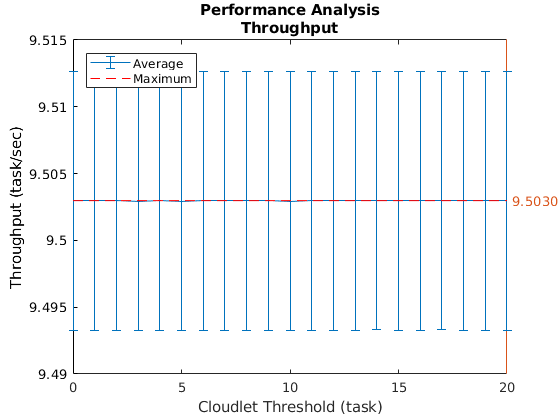
\includegraphics[width=\columnwidth]{fig/evaluation-performance-analysis-throughput}
	\caption{Performance analysis of the throughput as a function of the threshold $S$  with level of confidence $95\%$. The throughput is clearly threshold insensitive, with a constant mean value $E[X]\approx9.5030 \; task/sec$. The threshold $S*=2$ is a good choice}
	\label{fig:evaluation-performance-analysis-throughput}
\end{figure}

\begin{figure}
	\begin{center}
		\begin{tabular}{|c||c|c|}
			\hline
			$\mathbf{S}$ & $\mathbf{\mu(X)\pm\delta_{0.05}}$ & $\mathbf{\sigma(X)}$\\
			\hline
			$0$  & $9.50296\pm 0.00969$ & $0.03818 $ \\
			$1$  & $9.50295\pm 0.00969$ & $0.03818$ \\
			$\mathbf{2}$  & $\mathbf{9.50296\pm 0.00969}$ & $\mathbf{0.03816}$ \\
			$3$  & $9.50294\pm 0.00967$ & $0.03808$ \\
			$4$  & $9.50296\pm 0.00969$ & $0.03816$ \\
			$5$  & $9.50294\pm 0.00969$ & $0.03818$ \\
			$10$ & $9.50295\pm 0.00969$ & $0.03818$ \\
			$15$ & $9.50295\pm 0.00968$ & $0.03813$ \\
			$20$ & $9.50296\pm 0.00970$ & $0.03821$ \\
			\hline
		\end{tabular}
	\end{center}
	\caption{Performance analysis of the throughput as a function of the threshold $S$ with level of confidence $95\%$.}
	\label{tbl:evaluation-performance-analysis-throughput}
\end{figure}

\begin{figure}
	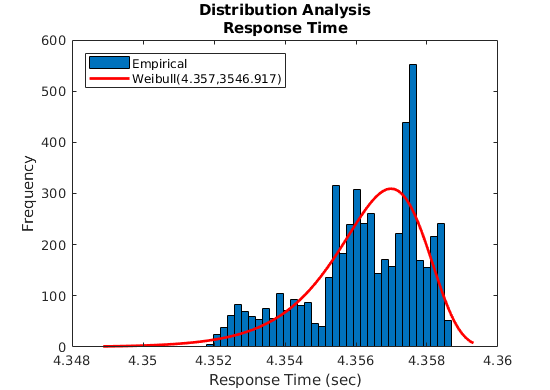
\includegraphics[width=\columnwidth]{fig/evaluation-distribution-analysis-response-time}
	\caption{Distribution analysis for response time with threshold $S=20$. The binning rule is Freedman-Diaconis Rule. The best fitting is the Weibull with parameters $A\approx4.357$ and $B\approx3546.917$.}
	\label{fig:evaluation-distribution-analysis-response-time}
\end{figure}

%%
% DISTRIBUTION ANALYSIS
%%
\subsection{Distribution Analysis}
\label{sec:evaluation-distribution-analysis}
\section{Usage}
\label{sec:usage}


In this Section we show how to configure and run experiments and some sample outputs to provide a better idea of what has been created.

The test of extremes for a custom random number generator produces the output shown in Figure~\ref{fig:usage-randomness-extremes} and can be executed with default configuration by running the script

\begin{lstlisting}
exp/random/randomness/extremes/main.py
\end{lstlisting}

\begin{figure}
	\centering
	\lstinputlisting{ext/randomness-extremes.txt}
	\caption{A sample output of the Test of Extremes.}
	\label{fig:usage-randomness-extremes}
\end{figure}

The test of Kolmogorov-Smirnov for a custom random number generator produces the output shown in Figure~\ref{fig:usage-randomness-kolmogorov-smirnov} and can be executed with default configuration by running the script

\begin{lstlisting}
exp/random/randomness/kolmogorov-smirnov/main.py
\end{lstlisting}

\begin{figure}
	\centering
	\lstinputlisting{ext/randomness-kolmogorov-smirnov.txt}
	\caption{A sample output of the Test of Kolmogorov-Smirnov.}
	\label{fig:usage-randomness-kolmogorov-smirnov}
\end{figure}

The simulation is configured providing a configuration YAML file as the one shown in Figure~\ref{fig:usage-simulation-configuration}, produces the output shown in Figure~\ref{fig:usage-simulation-output} and can be executed by running the script

\begin{lstlisting}
exp/simulation/performance/main.py
\end{lstlisting}

\begin{figure}
	\centering
	\lstinputlisting{ext/simulation-configuration.yaml}
	\caption{A sample configuration for a simulation experiment.}
	\label{fig:usage-simulation-configuration}
\end{figure}

\begin{figure}
	\centering
	\lstinputlisting{ext/simulation-output.txt}
	\caption{A sample output of a simulation experiment.}
	\label{fig:usage-simulation-output}
\end{figure}



\section{Conclusions}
\label{sec:conclusions}

%%
% SUMMARY
%%
In this work we propose a next-event simulator for a two-layer Cloud system with off-loading policy on class-partitioned workload, whose random components leverage a multi-stream Lehmer pseudo-random number generator.

%%
% CONCLUSIONS
%%
We may conclude that (i) our simulator returns experimental results that are consistent with the theoretical ones, (ii) the system can achieve the steady-state (iii) the choice of the threshold $S$ is critical for system performances and (iv) the adopted preemption policy allows to balance response time for classes of tasks with different service rates. 

%%
% IMPROVEMENTS
%%
Although our results are pretty satisfactory, the proposed solutions could certainly be improved and be subjected to a more in-depth analysis.
%
From an implementation point of view, the proposed solution should be ported from Python to C and leverage multi-threading to achieve better performances, e.g. to speed-up the algorithms to find suitable multipliers for modulus in 64-bit architectures and make faster simulations.
%
From an analysis point of view, the proposed random number generator should be tested more extensively. For example, we may (i) take into account more tests of randomness (ii) use a pseudo-random number generator with a 64-bit modulus and less number of streams.
%
Finally, the simulation model should be extended in order to 
(i) study the influence of different server selection policies, e.g. equity-selection, and 
(ii) achieve more performance evaluation goals, such as forecasting with respect to the variation of the arrival processes.


%*******************************************************************************
% Bibliography
%*******************************************************************************
\bibliographystyle{biblio}
\bibliography{./ref/biblio}

\end{document}
